% vim: ft=tex
\chapter{Scope}
The technical goals of this bachelor thesis include extending mindclue GmbH's
Roadster framework by adding features such as clustering, high availability and
transport security. This chapter outlines the general scope of this project.

\section{Motivation}
\subsection{Personal backgrounds}
To better understand our motivation, it might help to understand our personal
backgrounds first.

\textbf{Patrik Wenger} did his apprenticeship in computer science at Swisscom
Schweiz AG, and stayed work as a full-time employee for five more years
afterwards. In programming he's most fluent in \gls{ruby} and \gls{c}. During
the winter of 2015/2016, he created \gls{cztop} during leisure time because
there was no good Ruby binding for \gls{zmq}/\gls{czmq} available and a side
project of his demanded it. Fascinated with event-driven programming and
software design patterns such as the \gls{actor-model} (e.g. the
Celluloid\footnote{a concurrency framework for Ruby based on the actor model,
\url{https://github.com/celluloid/celluloid}} library on Ruby, or
Pony\footnote{a young programming language completely based on actors,
\url{http://www.ponylang.org}}, distributed computing and high availability
have long been part of his core interests, especially in conjunction with the
brilliant \zmq library. Having a passion for information security and modern
cryptography\footnote{such as \gls{nacl} or \gls{libsodium} as used by
\gls{zmq}}, especially in this post-Snowden era, this bachelor thesis couldn't
be a better match.

\textbf{Manuel Schuler} did his apprenticeship in computer science at Alcatel-Lucent AG.
The most projects during the apprenticeship or other companies involved network monitoring or
configuration automation. In programming he's most fluent in Node.js, Java and .NET. He
made several projects to keep his life simple. After a while he decided to start his own business.
Always keen on learning new things and the fact he often made similiar things like Patrik Wenger during his work
career motivated him to learn how Patrik did the things he did,
so he did not hestiate to join this bachelor theis at the first opportunity.

In essence, both students are thrilled to gain more experience in the following
fields and technologies:

\begin{itemize}
	\item Distributed Computing
	\item High Availability
	\item Information Security
	\item \gls{actor-model}
	\item \gls{zmq}
	\item \gls{ruby}
\end{itemize}

\subsection{Opportunities}
Coming from different backgrounds and having different levels of experience in
each of the above technologies, we can't wait to learn more about them and put
them to actual use. The fact that the product of this bachelor thesis is most
likely going to be used in the real world only adds to the excitement.

This bachelor thesis involves working with Ruby, the Actor Model, \zmq,
distributed computing with high availability, and state-of-the-art
cryptography. Furthermore, in case of successful completion of this thesis, the results will be used in real-world settings like the Ceneri
Base Tunnel. It is a huge opportunity for a solution completely based on free
and open-source software interacting with other industrial systems over open standards. The students, as well as the client, strongly believe
in customized solutions built on reusable, free open-source software.

In addition to that, we look at this bachelor thesis as an opportunity to
become more fluent in English, both written and spoken, as well as to improve
our skills in crafting scientific documents using {\LaTeX}.

Depending on how we perform together as a team, further collaboration might
result in the future, either between the students themselves, or between the
students and the client. Even if our paths will part, this project will
serve as a valuable reference for future job hunting.

Last but not least, we feel like Prof. Dr. Mehta is a respected and competent
teacher whose opinions we highly value. Due to his polite parlance, discussing
project matters, both of the management and the technical kind, has always been
an enrichment.

\subsection{Open-Source engagement}
Getting the chance to use \gls{cztop} and watch it perform definitely adds to
the motivation as well. Its software design has yet to be proven in more
serious settings.

Another personal goal is to create a reusable open-source library as a
byproduct. The intention is that the library makes certain \zmq-based
communication protocols readily available for other developers facing the same
problems.

\section{Initial Situation}

\subsection{mindclue GmbH}
The company mindclue GmbH, located in Ziegelbr\"ucke GL, provides its partner
REMTEC AG with complete \gls{SCADA}\footnote{SCADA software resides in level 2 of the enterprise levels (0--4) modeled by the \gls{isa95} standard, \url{https://en.wikipedia.org/wiki/Enterprise_control}} applications. These are then used to
supervise and control operation and safety equipment found in:
% ISA95 “levels”

\begin{itemize}
\item national freeways, e.g. emergency phones
\item tunnels, e.g. lights and ventilation
\item water supply systems
\item energy facilities
\item many other specialized fields
\end{itemize}

To build these customized applications, their in-house creation
Roadster, a next-generation SCADA framework, is used.

\subsection{Roadster}
Roadster is a SCADA framework written in Ruby. It was, and still
is, developed to produce next-generation SCADA applications to replace legacy
solutions based on its predecessor found in numerous tunnel
facilities in Switzerland.

A Roadster installation combines the following responsibilities:

\begin{itemize}
	\item interaction with subordinate field devices (monitoring \& controlling)
	\item persisting data (e.g. certain sensor data, and events)
	\item sophisticated alarm (\emph{case}) management
	\item providing a machine-to-machine interface to higher level systems
	\item providing a modern, customized web UI for interaction with operational and executive personnel
\end{itemize}

Among others, the field devices include various kinds of \glspl{PLC}\footnote{an example
is the SIMATIC S7-1500 by Siemens AG,
\url{http://w3.siemens.com/mcms/programmable-logic-controller/en/advanced-controller/s7-1500/Pages/default.aspx}}
as well as emergency call systems\footnote{an example is the NIS ComNode by Trans Data
Management AG,
\url{http://trans-data.com/en/k2-categories/item/149-niscomnode}}.
These are interacted with over numerous propietary and standardized protocols.

\subsubsection{System integration}
This section briefly describes the big picture of Roadster's place within
typical production environments and its relationship with other systems.

In some deployments, Roadster has no higher-level client systems, but is
operated as a standalone supervision and control system. In that case, the only
clients would be its human users. This usually applies to solutions delivered
to counties as opposed to solutions operating on a national level.

In other deployments, there are higher level systems which act as clients of a Roadster instance, communicating over
protocols including \gls{SOAP} and \gls{opc-ua}. Their purpose is to
collect and aggregate supervisory data from larger regions. At the top of the
hiearchy are the \gls{FEDRO} (German: \gls{ASTRA}) which combine the information of all
subsystems to provide a nationwide overview.

\begin{figure}[]
	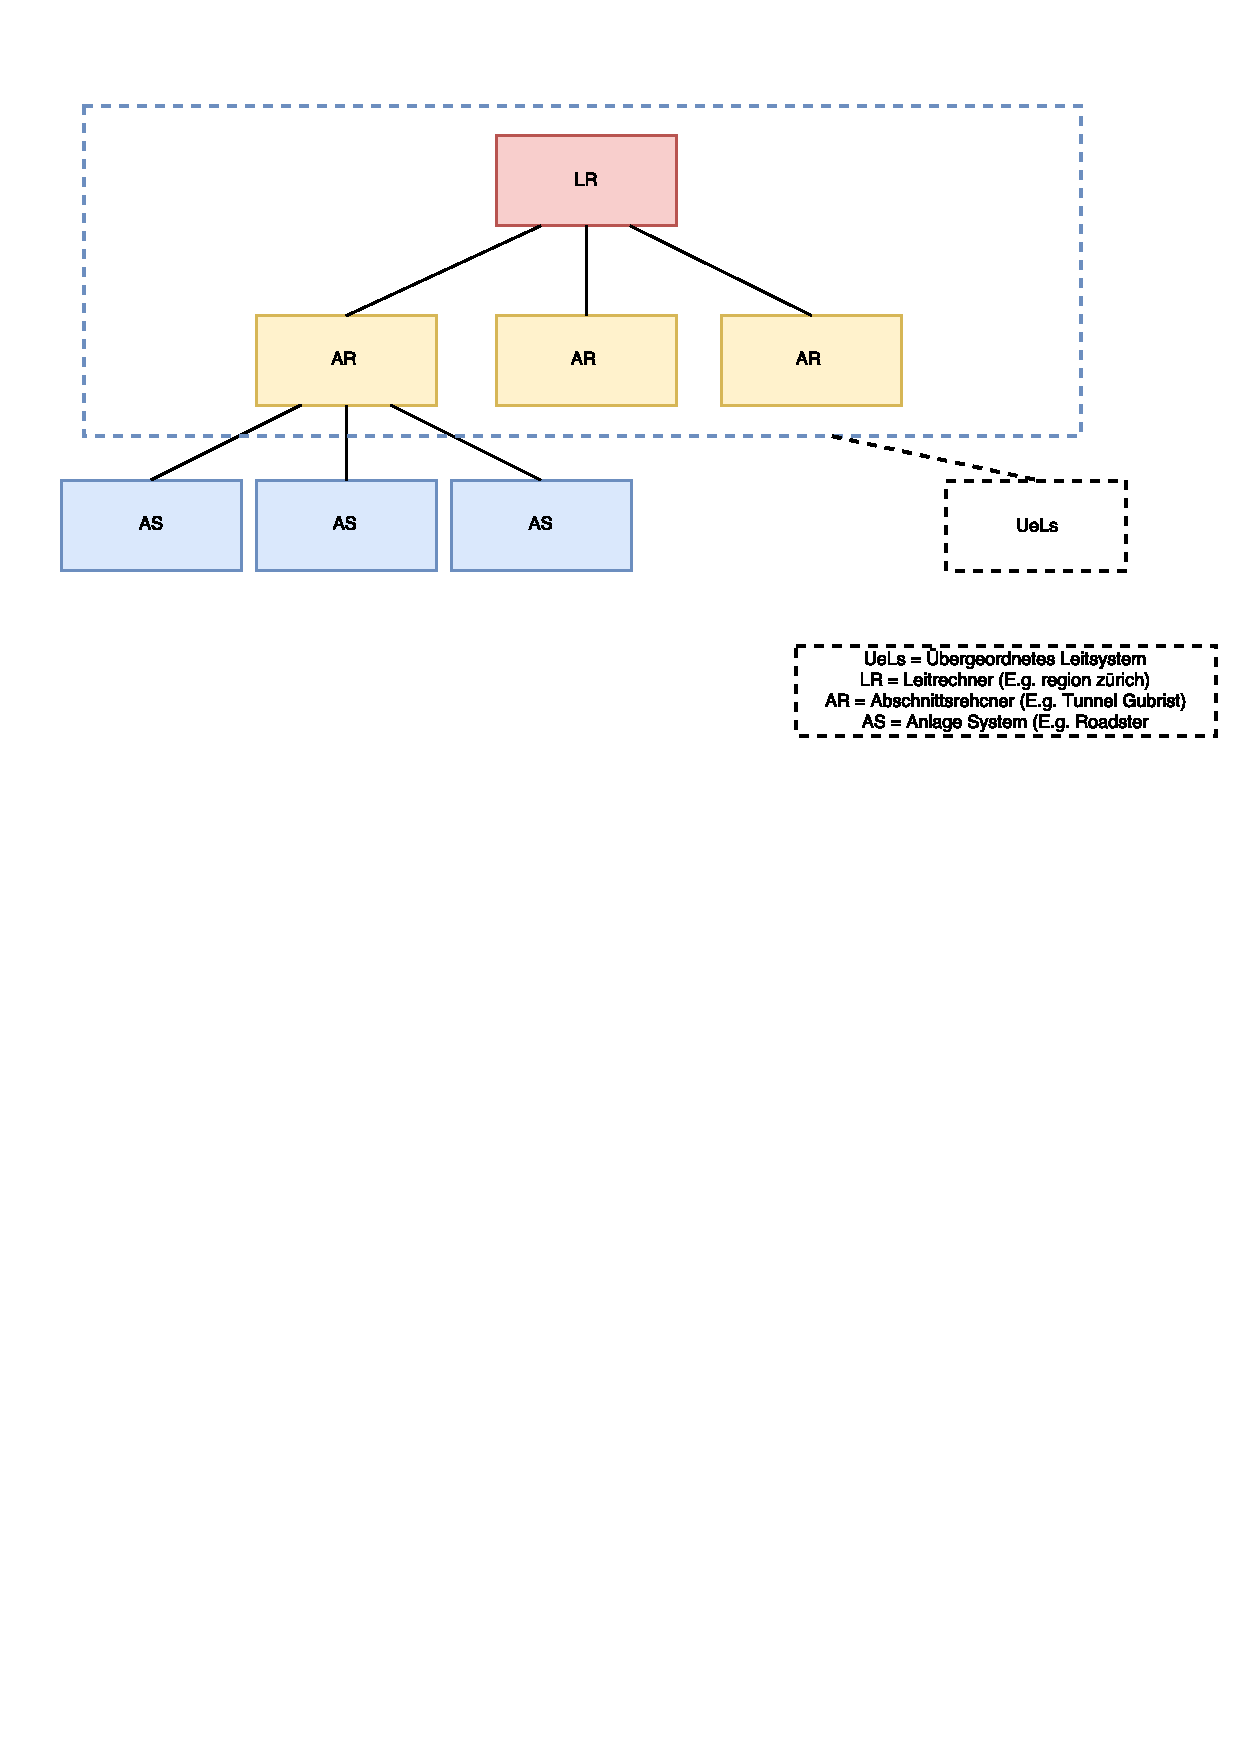
\includegraphics[width=\textwidth]{img/overall_system.pdf}
	\caption{Roadster's place within the overall system}
	\label{fig:roadster:overallsys}
\end{figure}

\autoref{fig:roadster:overallsys} illustrates the typical, overall system. The line
style meanings also apply to the remaining physical topology illustrations. The acronyms
used, which are part of the \gls{FEDRO} terminology, don't have official
English translations; not even the department itself was able to help with
translations on request, so they were left unchanged. A brief description
follows, from the bottom up:

\begin{description}
	\item [ Field devices: ] \hfill\\
	Field devices are various kinds of \glspl{PLC} and other subordinate systems
	used to supervise and control industrial processes. Communication with them
	happens over protocols such as \gls{modbus-tcp}, \gls{iec-104}, and
	\gls{opc-ua}.

	\item [ \gls{AS}: ] \hfill\\
	This is Roadster's domain, or of course the one of another product with similar
	functionality. An AS is responsible for one facility (e.g. emergency call system,
	lighting system, fire alarm system, video monitoring system, ventilation
	system, power supply system, train signaling system).

	\item [ \gls{AR}: ] \hfill\\
	The higher level system of the collection of all AS found in one larger
	facility such as a tunnel. With the results of this bachelor thesis, this
	\emph{could} be Roadster's domain as well.

	\item [ \gls{LR}: ] \hfill\\
	The higher level system of the collection of all AR found in a region such as
	Z\"urich. As with AR, this \emph{could} be Roadster's domain as well.

	\item [ \gls{LTA}: ] \hfill\\
	This collective term comprises both the levels of AR and LR. For
	simplicity and readability's sake, this will be referred to as
	\emph{client} for the remainder of this document.
\end{description}

\subsubsection{Typical hardware}
Roadster typically runs on entry-level rack server hardware powered by an
Intel\textregistered{} Xeon\textregistered{} processor, or industrial box PCs for smaller systems
commonly used for \gls{IoT} which are powered by more energy efficient processors
such as Intel\textregistered{} Core\textregistered{} and Intel\textregistered{}
Atom\texttrademark{}. The machines are usually equipped with 4 -- 6 GiB of main
memory and Gigabit Ethernet. For reliable systems without any moving parts, an
industrial grade \gls{SSD} or two (in a software \gls{RAID} level 1 setup) are used.

\subsection{\zmq}
To understand Roadster's architecture and the rest of this document, it's
helpful to understand the basics of \zmq first. This is a brief introduction to
\zmq for the unfamiliar reader. What follows is a quote from the \gls{zguide}
which does a fairly good job at describing \zmq in a 100 words:

\begin{quote}
``ZeroMQ (also known as \zmq, 0MQ, or zmq) looks like an embeddable networking
library but acts like a concurrency framework. It gives you sockets that carry
atomic messages across various transports like in-process, inter-process, TCP,
and multicast. You can connect sockets N-to-N with patterns like fan-out,
pub-sub, task distribution, and request-reply. It's fast enough to be the
fabric for clustered products. Its asynchronous I/O model gives you scalable
multicore applications, built as asynchronous message-processing tasks. It has
a score of language APIs and runs on most operating systems.  ZeroMQ is from
iMatix and is LGPLv3 open source.''
\end{quote}

For a more detailed introduction, see \autoref{ch:zmq}.

Roadster uses \zmq to carry messages between its processes. The
library\footnote{The library is called \emph{ffi-rzmq} and is hosted on
\url{https://github.com/chuckremes/ffi-rzmq}} it uses to interface with \zmq is
unmaintained and doesn't support recent versions of \zmq (namely the ones
supporting encryption).

\subsection{Software architecture}
As mentioned earlier, Roadster is event-driven\footnote{\url{https://en.wikipedia.org/wiki/Event-driven_programming}} and built on the Actor model, meaning it exhibits a
shared-nothing architecture. Each Roadster node runs a number of Ruby processes
which communicate via \zmq sockets. The key here is communication:

\begin{quote}
``Don't communicate by sharing state; share state by communicating.''
\end{quote}

Running multiple, loosely coupled processes (actors) allows leveraging the full
potential of modern multi-core processors, while avoiding a whole class of
traditional concurrency problems.

Every Roadster node runs a group of actors:

\begin{description}
	\item [CORE:]\hfill\\
		It is responsible to start the other actors. It also plays a
		key role in keeping state in all actors synchronized, being the
		source of truth.

	\item [COMM:]\hfill\\
		A bunch of COMM actors communicate with the outside world of a
		node. It typically either acts as a client of various kinds of
		field devices, or as a server to the client. To do so, it
		utilizes the appropriate adapter which is defined by the static
		configuration of a Roadster application. These adapters
		implement communication protocols used to communication with
		field devices, but also to client systems (e.g. over
		\gls{opc-ua}). The webserver\footnote{The webserver \emph{Thin}
		is utilized, see \url{http://code.macournoyer.com/thin/}} for the
		web UI also runs in a COMM actor.

	\item [STORAGE:]\hfill\\
		This actor is used when information needs to be persisted, such
		as time series or event journals. It's the interface to a
		key-value store.

	\item [LOGGER:]\hfill\\
		This actor collects logging data and sends it to whatever
		target is configured, be it \gls{stdout}, a file, or a syslog server.
\end{description}

\autoref{fig:roadster:arch} illustrates Roadster's architecture.

\begin{figure}[]
	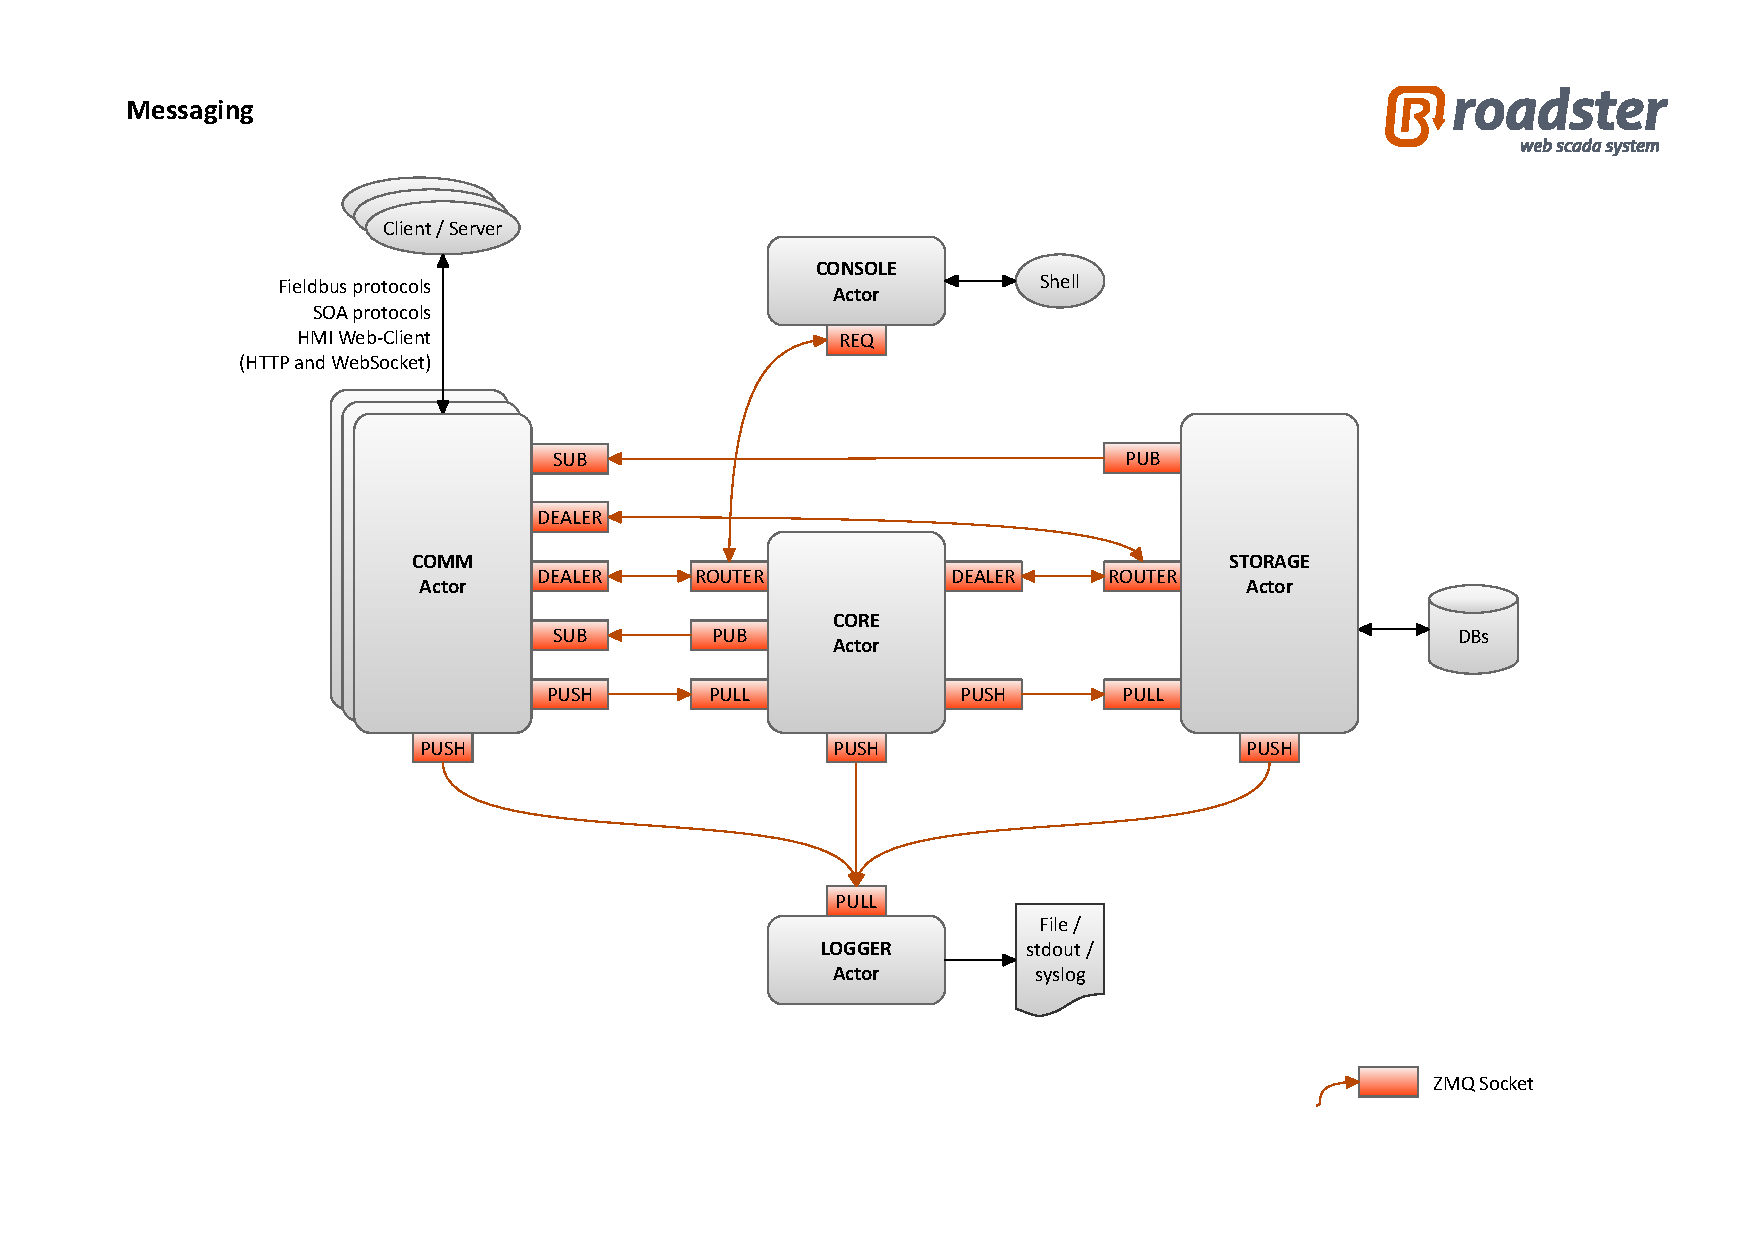
\includegraphics[trim=4cm 2cm 3.5cm 2.8cm, clip=true, width=\textwidth]{img/roadster_arch.pdf}
	\source{Andy Rohr}
	\caption{Roadster's software architecture}
	\label{fig:roadster:arch}
\end{figure}

\subsubsection{Communication Layers}
The communication architecture in Roadster consists of three layers, as
illustrated in \autoref{fig:roadster:layers}. The following list briefly
explains the layers from top (most abstracted) to bottom:

\begin{description}
	\item [Engine layer:]\hfill\\
		Here is the business logic of Roadster, e.g. the \gls{DIM},
		user authentication, adapters for different devices, the web
		\gls{UI}, etc.

	\item [Messaging layer:]\hfill\\
		The \gls{RMP} reside here and implement essential protocols used
		for logging, state synchronization, commands, application controlling,
		and storage. They're explained below in \autoref{sec:rmp}.

	\item [Reactor layer:]\hfill\\
		This layer forms the base, which is where the \zmq sockets and
		\glspl{websocket} are utilized. It is powered by an
		event-loop\footnote{EventMachine is used as a high-performance event-loop to
		manage large numbers of sockets and timers,
		\url{https://github.com/eventmachine/eventmachine}}. Sockets used by COMM actors
		to communicate with various field devices are also integrated into this
		event-loop.
\end{description}

\begin{figure}[]
	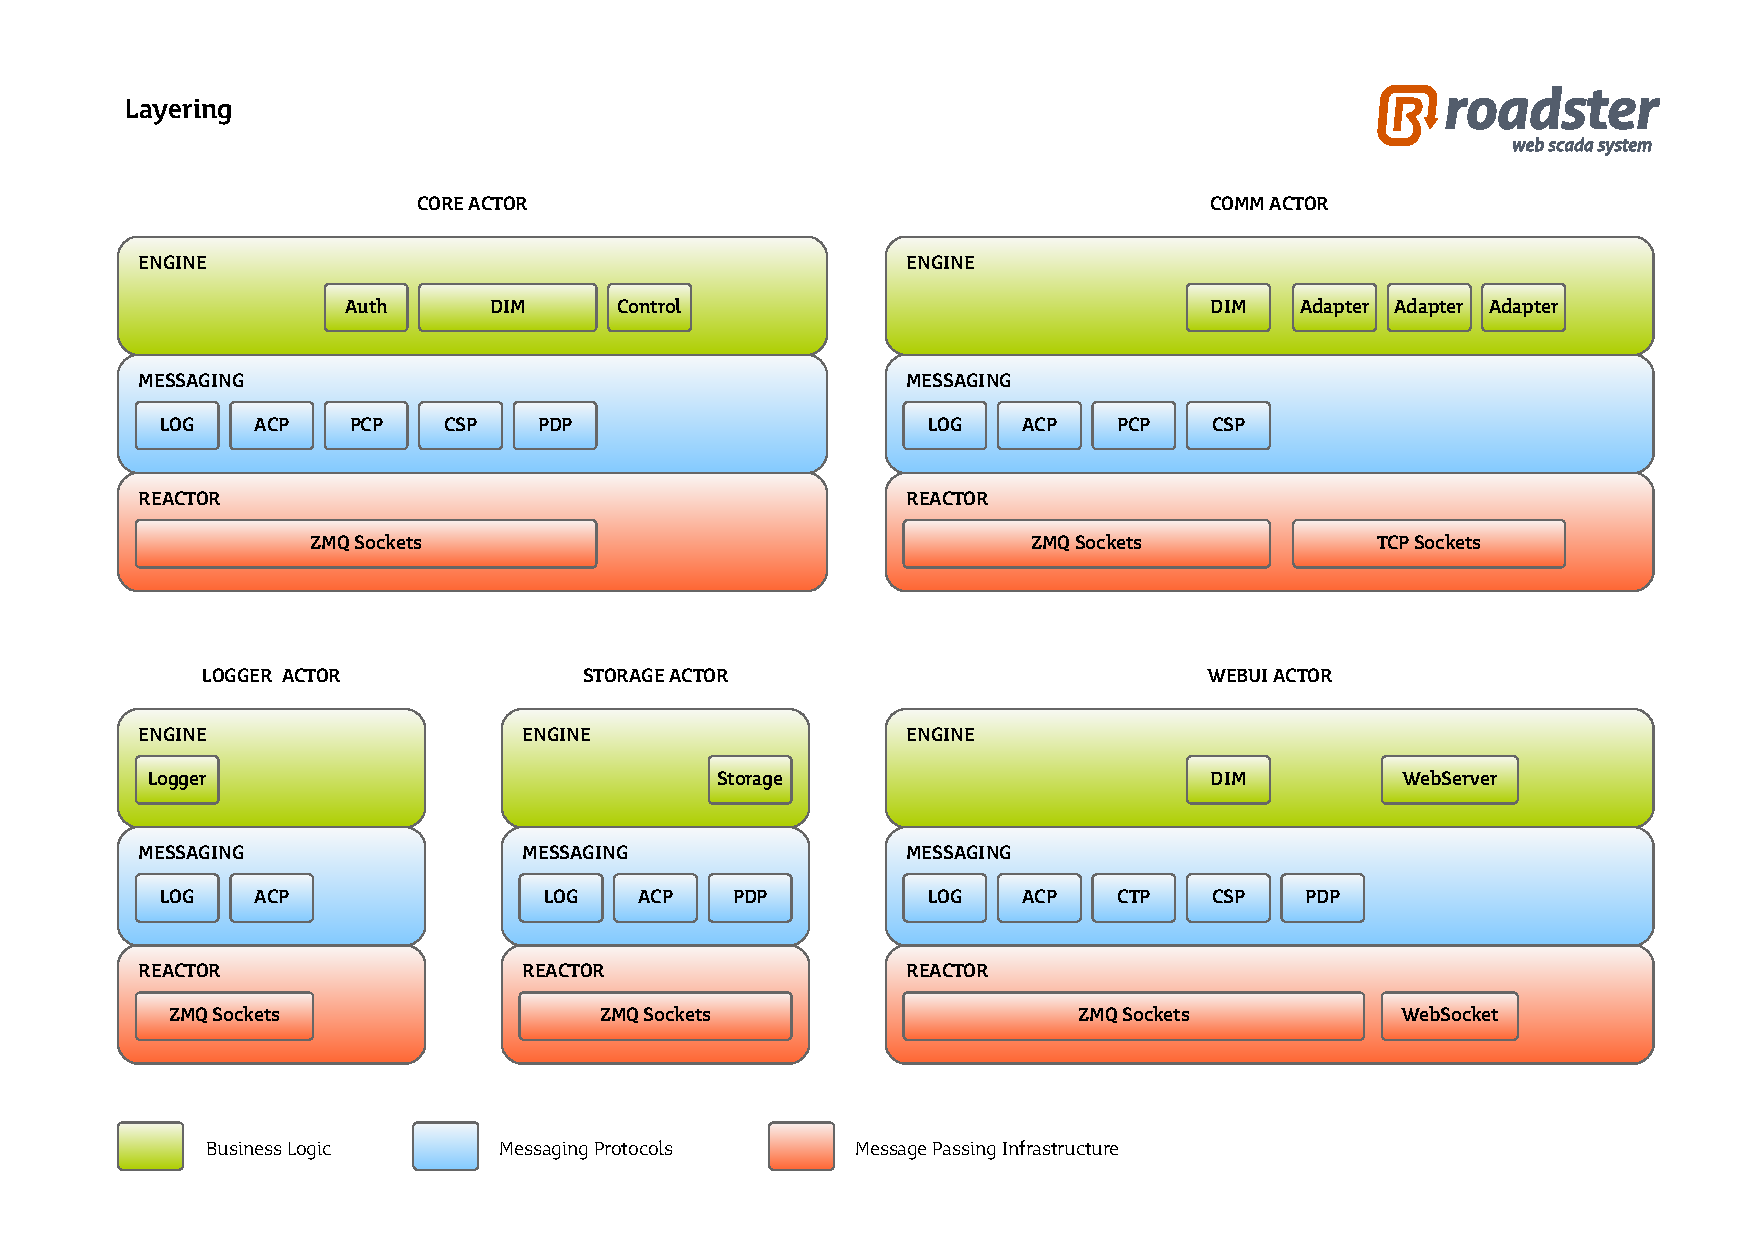
\includegraphics[trim=1.95cm 2.5cm 1.65cm 2.8cm, clip=true, width=\textwidth]{img/roadster_layering.pdf}
	\source{Andy Rohr}
	\caption{Roadster's communication layers}
	\label{fig:roadster:layers}
\end{figure}

\subsubsection{RMP}\label{sec:rmp}
The \gls{RMP} are a collection of protocols implemented and used by Roadster
internally. They reside in the messaging communication layer, and include:

\begin{description}
	\item [\gls{CSP}:]\hfill\\
		Used to synchronize state between the actors.
	\item [\gls{ACP}:]\hfill\\
		Used to control the application state, e.g. shutdown.
	\item [\gls{PDP}:]\hfill\\
		Used when data needs to be persisted.
	\item [\gls{SMP}:]\hfill\\
		Used to suppress the generation of certain \glspl{case}, e.g.
		when a sensor is defect and repeatedly causes cases.
	\item [\gls{PCP}:]\hfill\\
		Used for asynchronous command execution via COMM peers with feedback.
	\item [\gls{LOG}:]\hfill\\
		Used for system logging.
\end{description}

Every actor in Roadster uses a subset of these protocols to perform its job.

Passing messages from actor to actor, which are nothing but serialized Ruby
objects, happens in one of two modes:
\begin{description}
\item [Fire \& Forget:]\hfill\\
No guarantee of correct processing, e.g. DIM updates from COMM to CORE. This
doesn't mean there are no other mechanisms in place to ensure reliability.

\item [Dialog:]\hfill\\
An immediate answer is expected, e.g. when creating a user
session. Sending a message like this looks like it's a synchronous call, even
though it's handled asynchronously under the hood\footnote{This is done by
wrapping the affected code in a Ruby \rb{Fiber}, which is similar to a thread
but allows for cooperative scheduling as opposed to preemtive.} Any protocol
can make use of this primitive.
\end{description}

\subsubsection{DIM}
The \acrfull{DIM} is a tree data structure that lives inside every actor of a Roadster
node. Every actor builds it when starting up by reading the configuration
files available to all actors.

The DIM consists of static objects and dynamic objects. The dynamic
objects\footnote{Namely instances of the meta-model classes \rb{Case},
\rb{DataItem}, and \rb{Session}} can be updated. The updates are then
replicated across all actors to keep the DIM synchronized. This works by
marking the updated object dirty\footnote{It is marked dirty by setting its
\rb{@lifecycle_state = "updated"}} so it is subsequently replicated via the
\gls{CSP}. \autoref{fig:roadster:meta-model} illustrates the class diagram of
all the classes whose instances constitute the DIM.

\begin{figure}[]
	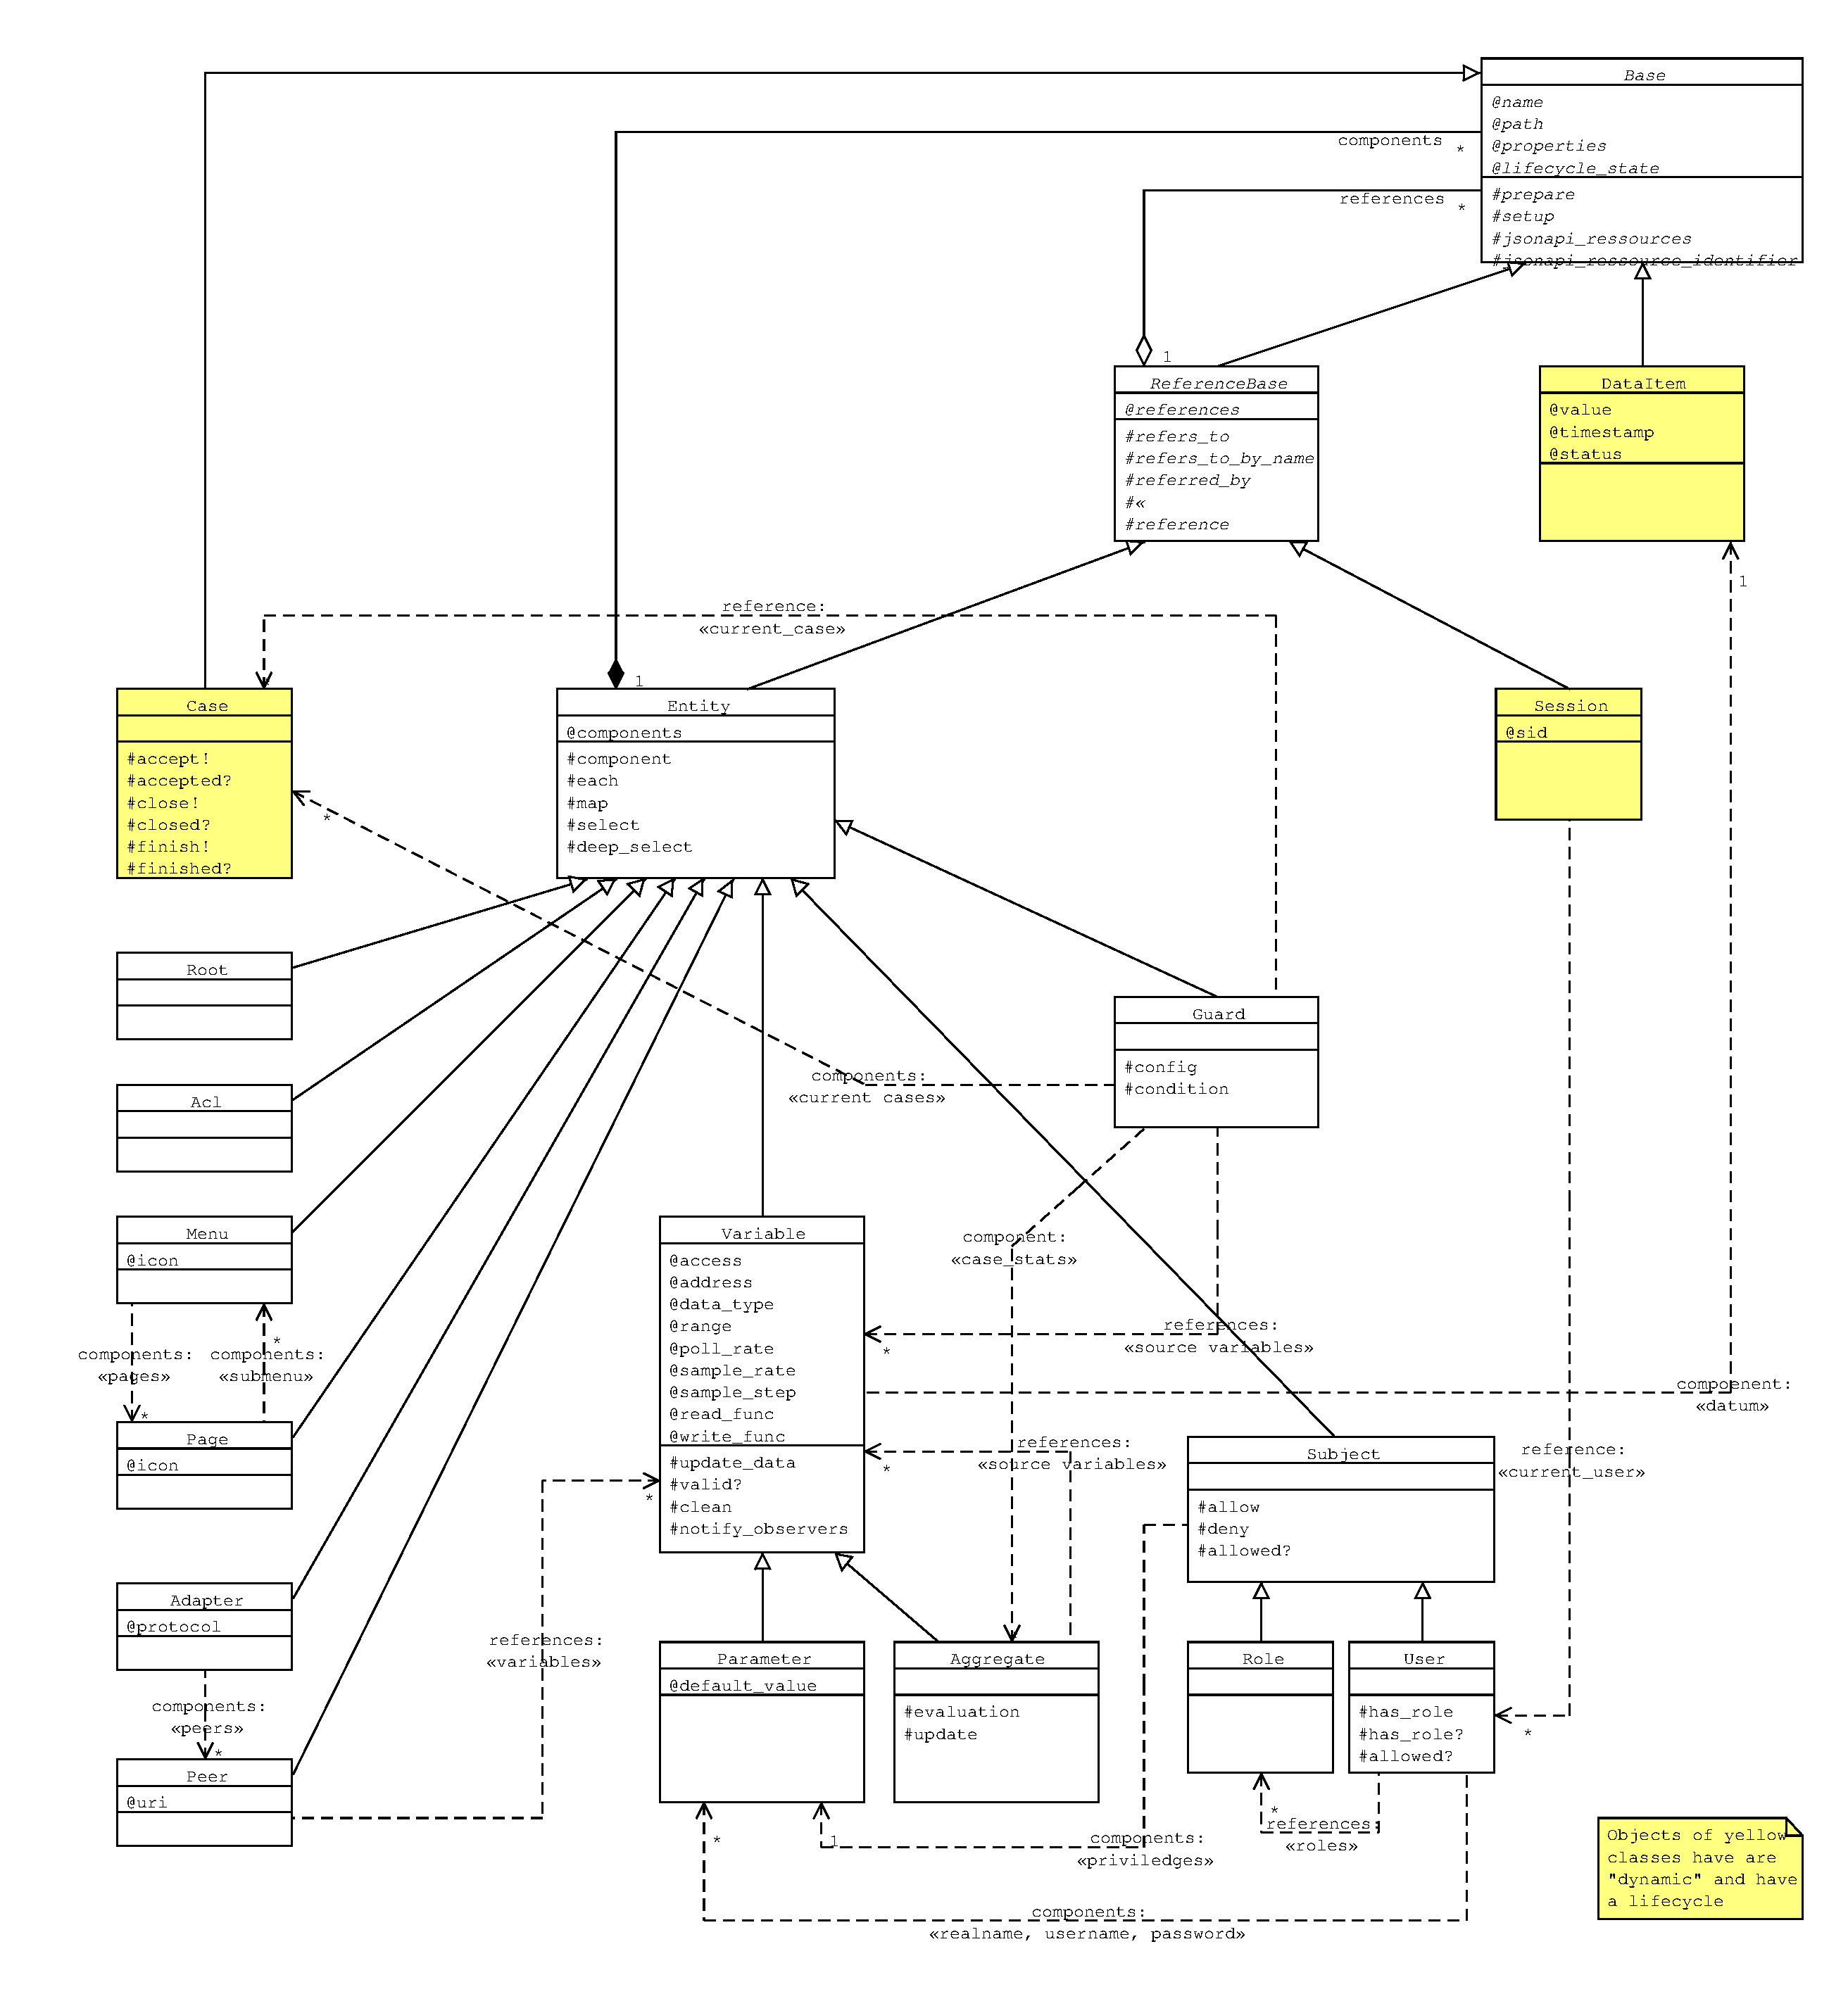
\includegraphics[trim=1.5cm 1cm 1cm 1cm, clip=true, width=0.9\textwidth]{img/meta_model.pdf}
	\source{Andy Rohr}
	\caption{Class diagram for Roadster's meta model used in the DIM}
	\label{fig:roadster:meta-model}
\end{figure}

\subsubsection{Existing CSP in a nutshell}
\emph{This is a brief introduction/refresher for the Clone State Pattern
implemented by Roadster, which is used for the DIM synchronization. Although Roadster actually sends serialized instances
of CSP message classes to fulfill this protocol, for better readability the
\gls{zguide}'s canonical nomenclature of \gls{clone-pattern} messages will be used.}

The existing \acrfull{CSP} is closely related to the \gls{clone-pattern} from the \gls{zguide}. Its
goal is to keep a state (a list of key-value pairs) in sync across a set of
participants. To greatly reduce the complexity, it's not decentralized: There's
a server part which serves as the single source of truth.

The server uses a ROUTER, a PULL, and a PUB socket; each client a DEALER, a
PUSH, and a SUB socket. The protocol consists of three distinct messages flows:

\begin{description}
	\item [Snapshots:]
		Requesting and receiving the complete, current snapshot of the
		state (all key-value pairs). This happens via a
		ROUTER/DEALER pair of sockets. The request message consists solely of
		the humorously named ICANHAZ command. The response is the
		complete set of KVSET messages so a late-joining (or previously
		disconnected) client can rebuild the current snapshot.

	\item [Upstream updates:]
		Updates always originate from clients and are sent to the
		server via a PUSH/PULL pair of sockets. These are KVSET messages.

	\item [Downstream updates:]
		After being applied to the server's copy of the state,
		updates get a sequence number and are published back to all
		clients. This happens via the PUB socket and
		uses KVPUB messages.
\end{description}

By making all updates go through the server, a total order is enforced,
which is crucial to keep the state consistent across all clients.

To avoid risking a gap between requesting the current snapshot and subscribing
to updates, a client actually subscribes to the updates first, then gets the
snapshot, and then starts reading the updates from the socket (which has been
queueing updates in the meantime, if any). Updates that are older or the same
age as the received snapshot are skipped, and only successive updates are
applied (tested by comparing the sequence numbers).

Because message loss via the third message flow (PUB-SUB) is unlikely but
theoretically possible, the client checks for gaps in the sequence number of
each KVPUB message. If a gap is detected, the current state is discarded and a
complete resynchronization happens. This is brutal, but is very simple and thus
robust; there's no complexity that would leave room for nasty corner cases.

A feature described in the \gls{zguide}, but not implemented in Roadster as of
this writing, are subtrees.
Keys can be treated hierarchically (e.g. \sh{topic.subtopic.key}) and thus, a
client can optionally subscribe to only a particular subtree. This is useful
when the number of client grows and not all of the state needs to be on every
client. In that case, the topic of interest is sent by the client along with
the ICANHAZ message.

% TODO: add illustration

\subsubsection{Persisted data}
Certain data on a Roadster node is persisted, which is done by the STORAGE
actor. Different data goes into different \gls{tc} database files, including:

\begin{description}
	\item [ Event journal: ] \hfill\\
		This is is a history of all cases (alarms), including the ones
		that have been confirmed and thus removed from the DIM. It
		resides in a \gls{tc} \emph{table} database, where the key is a
		\gls{UUID}, one of the columns (attributes) is the timestamp of
		the case, and another one is the actual, serialized \rb{Case}
		object. Objects in this database can be modified, e.g. when a
		pending case is confimed.

	\item [ Time series: ] \hfill\\
		This is a pure key-value store that stores samples of sensor
		data from field devices. Only the most recent value of these
		are actually kept in the DIM. One file per series is used. The
		timestamp is part of the key.

	\item [ Parameters: ] \hfill\\
		Parameters are the third and last kind of persisted data in
		Roadster. Parameters are typically changed by a user. Each
		parameter is backed by a default value from the configuration,
		which is used as long as there is no actual corresponding value
		set or read from the database. Credentials for users of the UI
		are an example parameters.
\end{description}

\section{Goals}
% TODO preprocessed mandatory goals
% TODO retrospective, diff with initial goals

To summarize the mandatory goals from the Task Description in \autoref{ch:task-desc}:

\begin{enumerate}
	\item Getting familiar with Roadster
	\item Extending the communication protocols to support federation of
		multiple nodes
	\item Extending the communication protocols to allow high availability
		clusters of two peer nodes
\end{enumerate}

The optional goals are:

\begin{enumerate}
	\item Encryption of the communication
	\item Providing of the highly available \gls{opc-ua} server interface
\end{enumerate}

\subsection{Additional goals}
The following goals were not explicitly part of the original task description,
but developed during the elaboration phase out of interest in the technical
matter.

\subsubsection{Security concerns of SCADA applications}
Secure inter-node communication within a Roadster federation is important to
mitigate common security concerns with SCADA systems which are becoming more
and more open due to standardization. To quote \cite[Security issues]{wp:scada}
wikipedia:

\begin{quote}
``In particular, security researchers are concerned about:
	\begin{itemize}
		\item the lack of concern about security and authentication in
			the design, deployment and operation of some existing
			SCADA networks
		\item the belief that SCADA systems have the benefit of
			security through obscurity through the use of
			specialized protocols and proprietary interfaces
		\item the belief that SCADA networks are secure because they
			are physically secured
		\item the belief that SCADA networks are secure because they
			are disconnected from the Internet.''
	\end{itemize}
\end{quote}

The goal is to provide a framework that makes it trivial to provide reasonably
secure SCADA applications which are assumed to be running on insecure networks.

\subsubsection{Fallacies of distributed computing}
At this place, it is worth noting the common fallacies encountered in
distributed computing, as explained on \cite{dcomp:fallacies}.

% TODO: briefly explain these, without our particular solutions to them

\begin{description}
	\item [The network is reliable.] \hfill\\
		Network outages need to be embraced and handled with
		appropriate error-handling to avoid stalls, permanent
		resource consumption, and the need for manual restarts.

	\item [Latency is zero.] \hfill\\
		The ignorance of network latency and packet loss can lead to
		wasted bandwidth when traffic is unbounded. Depending on the
		application, assuming instant packet delivery could lead to
		timing issues like hanging user interfaces, especially if some
		nodes aren't in the same LAN.

	\item [Bandwidth is infinite.] \hfill\\
		Trying to send too much information can lead to bottlenecks,
		slow applications, and simply wasted bandwidth.

	\item [The network is secure.] \hfill\\
		This touches the subject mentioned before. SCADA applications
		often run in isolated networks, at least not directly reachable
		from the internet, but that doesn't make them secure. Threats
		from within are real and thus one cannot assume a network is
		secure.

	\item [Topology doesn't change.] \hfill\\
		Topology changes constantly. Services are added and removed. An
		application must not depend on specific endpoints or routes.

	\item [There is one administrator.] \hfill\\
		The overhead introduced by having coordinate multiple
		administrators is not negilible.

	\item [Transport cost is zero.] \hfill\\
		% TODO

	\item [The network is homogeneous.] \hfill\\
		% TODO

\end{description}

The goal is to conduct this thesis with the above fallacies in mind and embrace
them in our solution.
